
\documentclass[titlepage,12pt]{article}
%\usepackage{fullpage}
\usepackage[hmargin=2cm,vmargin=3cm]{geometry}
\usepackage{cite}
\usepackage{gensymb}
\usepackage{booktabs}
\usepackage{graphicx}
\usepackage{setspace}
\usepackage{fixltx2e}
\usepackage{amssymb}
\usepackage{verbatim}
\usepackage{float}


\begin{document}
\begin{titlepage}
\begin{center}

{\large Department of Electrical Engineering}\\
{\Large The Cooper Union for the Advancement of Science \& Art} \\[7cm]



% Title
{ \huge \bfseries System Calls and Error Reporting}\\[1.5cm]


{\Large by\\[.5cm]}
{\large Benjamin Schenker}
\end{center}



\vfill






{\large Advisor: Prof. J Hakner \hfill ECE 357 Problem 1}

\begin{center} 
{\large Fall 2013}
\end{center}


\end{titlepage}
\doublespacing
\section{Introduction}
A simple C program was written to utilize UNIX system calls for file I/O and properly handle and report error conditions.  A script was then written in MATLAB to measure the throughput of the program for various buffer sizes.
\section{Results}
\begin{figure}[H]
\centering
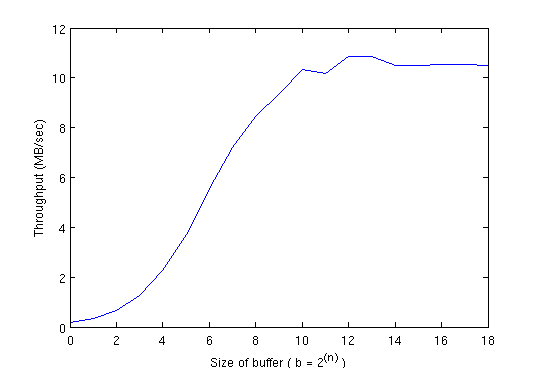
\includegraphics[scale = 1.2]{chart.png}
\caption{Throughput of copycat with varying buffer size}
\label{chart}
\end{figure}

The script executed the program taking input from a static 2.2MB file of random bytes (previously drawn from /dev/urandom) and copying it to a separate file.  The only change between calls was the specified buffer size.  As is shown in figure \ref{chart}, the throughput is quite low for very small buffers but there is only minor gain once the buffer is larger than 1024 bytes.  
\section{Analysis}
There are many reasons that the buffer size would affect the throughput in this way.  One major contributor is that a smaller buffer requires more system calls, which can be quite time consuming.  For example when the buffer size is 1 byte, the program has to make 4.4 million system calls (a read and a write for each byte).  This explains the very noticable 12 second runtime for the program using a 1 byte buffer.  This effect is mitigated as the buffer size increases such that the frequency of the system calls is closer to that of the normal timer interrupt.  
\section{Testing Environment}
The tests were performed on a Dell Vostro with an intel Core i7 processor running ArchLinux (in the SeniorLab).   The OS uses AFS and ACLs instead of UNIX permissions.  While it ignores group and world UNIX permissions AFS does utilize the user level UNIX permissions.  Thus user level permissions were modified to test the error handling of the program.  
\section{Conclusion}
The project was successfuly completed and the effect of the buffer size on the throughtput was measured and discussed.  




\end{document}
